\label{anhang}

\section{Paketdokumentationen}

Links zu den Dokumentationen der verwendeten Pakete.

\begin{itemize}
    \item inputenc: \url{http://ctan.org/pkg/inputenc}
    \item babel: \url{http://ctan.org/pkg/babel}
    \item amsmath: \url{http://ctan.org/pkg/amsmath}
    \item xifthen: \url{http://ctan.org/pkg/xifthen}
    \item graphicx: \url{http://ctan.org/pkg/graphicx}
    \item microtype: \url{http://ctan.org/pkg/microtype} \\
	    bzw. \url{http://ctan.org/pkg/microtype-de}
    \item units: \url{http://ctan.org/pkg/units}
    \item setspace: \url{http://ctan.org/pkg/setspace}
    \item hyperref: \url{http://ctan.org/pkg/hyperref}
    \item caption: \url{http://ctan.org/pkg/caption}
    \item cite: \url{http://ctan.org/pkg/cite}
    \item scrlayer-scrpage: \url{http://ctan.org/pkg/scrlayer-scrpage}
    \item array: \url{http://ctan.org/pkg/array}
    \item dcolumn: \url{http://ctan.org/pkg/dcolumn}
\end{itemize}

Leider wird nicht für jedes Pakete eine Dokumentation angeboten, sondern ihr findet dann nur Informationen zum Autor des Paketes vor.

\clearpage

\subsection{Texmaker einrichten}\label{sec:texmaker}

Als Editor bevorzuge ich Texmaker, da dieser alle wichtigen Funktionen bietet und unter vier verschiedenen Betriebssystemen (Windows, Linux, MacOsX und sogar OS/2) ausführbar ist. Bei der folgenden Anleitung beziehe ich mich auf die \LaTeX-Umgebung, welche vom ZIV der Uni Münster zur Verfügung gestellt wird. Darauf hat man Zugriff, wenn man sich im Netzwerk der Uni befindet (auch per VPN).


\subsubsection{\LaTeX-Befehle einrichten}\label{sec:texmaker_conf}

\begin{figure}[bh]
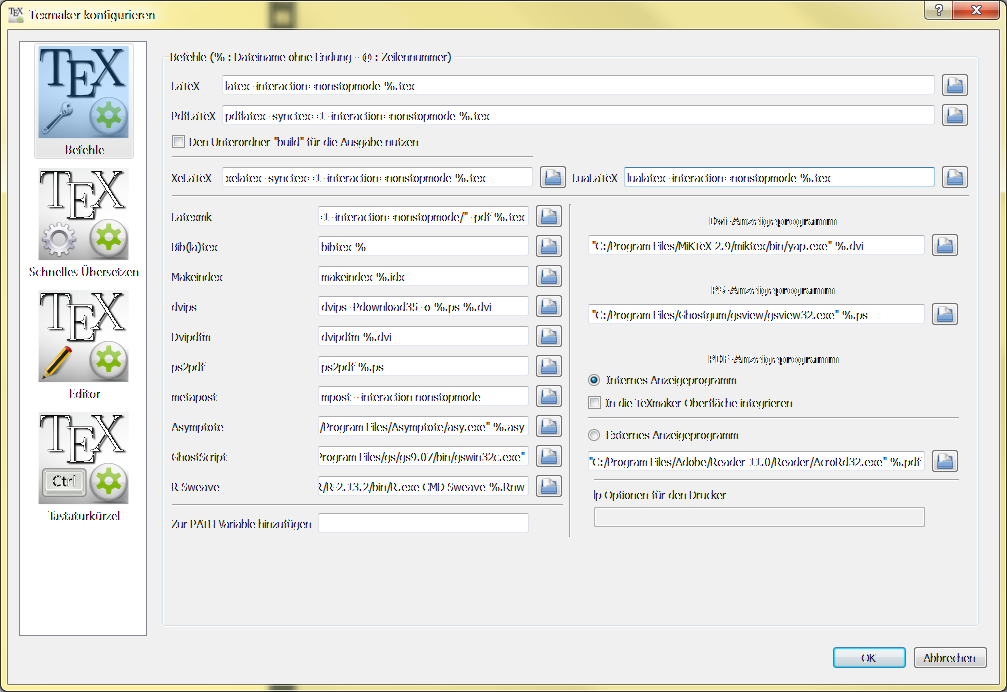
\includegraphics[width=\textwidth]{Bilder/Texmaker_konfigurieren.png} 
\caption{Dialog zum einrichten von Texmaker (hier Version 4.2)}
\label{img:texmaker_conf}
\end{figure}

Abbildung \ref{img:texmaker_conf} zeigt den Dialog zum Einrichten von Texmaker. Dieser ist über den Menüeintrag \verb+Optionen > Texmaker konfigurieren+ zu erreichen. Beim ersten Start stehen hier noch die Befehle ohne Pfadangabe. Ist MiKTex, oder texlive auf dem eigenen PC installiert, dann muss hier nichts mehr geändert werden. Anders sieht es an einem PC in der Uni aus. texlive ist auf einem zentralen Netzlaufwerk installiert, das eigene Betriebssystem weiß jedoch nichts davon. Man könnte jetzt dem Betriebssystem texlive über die Umgebungsvariable PATH bekannt machen, aber ich möchte einen anderen Weg vorführen. Dazu ruft man \verb+Optionen > Texmaker konfigurieren+ auf und es wird der in Abbildung \ref{img:texmaker_conf} zu sehende Dialog angezeigt. Bei allen benötigten \LaTeX-Befehlen (das sind eigentlich nur PdfLaTeX und Bib(la)tex) muss der Pfad angepasst werden. Dazu fügt man am Anfang des entsprechenden Textfeldes \verb+\\wwuappl2\W\TeX\texlive2010\bin\win32+ ein. Aus 

\begin{verbatim}
   pdflatex -synctex=1 -interaction=nonstopmode %.tex
\end{verbatim}

wird dadurch

\begin{verbatim}
   \\wwuappl2\W\TeX\texlive2010\bin\win32\pdflatex -synctex=1
      -interaction=nonstopmode %.tex
\end{verbatim}

\subsubsection{Schnelles Übersetzen einrichten}

\begin{figure}[bh]
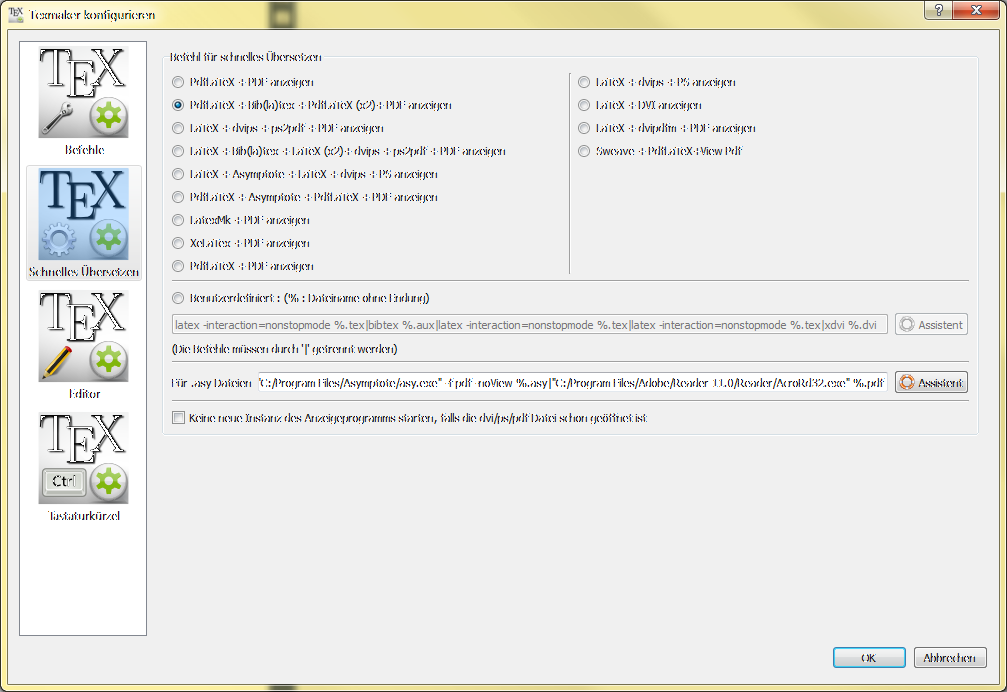
\includegraphics[width=\textwidth]{Bilder/Texmaker_konfigurieren2.png} 
\caption{Dialog zum einrichten von Texmaker (hier Version 4.2)}
\label{texmaker_konf2}
\end{figure}

Ruft man Schnelles Übersetzen auf (z.\,B. über die Toolbar, oder mit der Taste [F1]), dann wird PdfLaTeX einmal ausgeführt und anschließend die erzeugte PDF-Datei in Texmaler angezeigt. Hat sich das Inhaltsverzeichnis seid dem letzten Aufruf von PdfLaTeX verändert, oder sind neue Verweise eingefügt worden, dann fehlen diese Änderungen in der PDF-Datei. Deshalb ist es sinnvoll von  PdfLaTeX + PDF anzeigen auf PdfLaTeX + Bib(La)TeX + PdfLaTeX (2x) + PDF anzeigen umzustellen. Dazu ruft man \verb+Optionen > Texmaker konfigurieren+ auf und selektiert auf der linken Seite Schnelles Übersetzen (siehe Abblidung \ref{texmaker_konf2}). Dort kann man neben den genannten Optionen noch viele weitere auswählen.